% Options for packages loaded elsewhere
\PassOptionsToPackage{unicode}{hyperref}
\PassOptionsToPackage{hyphens}{url}
%
\documentclass[
  11pt,
  ignorenonframetext,
  aspectratio=169,
  c]{beamer}
\usepackage{pgfpages}
\setbeamertemplate{caption}[numbered]
\setbeamertemplate{caption label separator}{: }
\setbeamercolor{caption name}{fg=normal text.fg}
\beamertemplatenavigationsymbolshorizontal
% Prevent slide breaks in the middle of a paragraph
\widowpenalties 1 10000
\raggedbottom
\setbeamertemplate{part page}{
  \centering
  \begin{beamercolorbox}[sep=16pt,center]{part title}
    \usebeamerfont{part title}\insertpart\par
  \end{beamercolorbox}
}
\setbeamertemplate{section page}{
  \centering
  \begin{beamercolorbox}[sep=12pt,center]{part title}
    \usebeamerfont{section title}\insertsection\par
  \end{beamercolorbox}
}
\setbeamertemplate{subsection page}{
  \centering
  \begin{beamercolorbox}[sep=8pt,center]{part title}
    \usebeamerfont{subsection title}\insertsubsection\par
  \end{beamercolorbox}
}
\AtBeginPart{
  \frame{\partpage}
}
\AtBeginSection{
  \ifbibliography
  \else
    \frame{\sectionpage}
  \fi
}
\AtBeginSubsection{
  \frame{\subsectionpage}
}

\usepackage{amsmath,amssymb}
\usepackage{lmodern}
\usepackage{iftex}
\ifPDFTeX
  \usepackage[T1]{fontenc}
  \usepackage[utf8]{inputenc}
  \usepackage{textcomp} % provide euro and other symbols
\else % if luatex or xetex
  \usepackage{unicode-math}
  \defaultfontfeatures{Scale=MatchLowercase}
  \defaultfontfeatures[\rmfamily]{Ligatures=TeX,Scale=1}
\fi
\usetheme[]{Luebeck}
\usecolortheme{beaver}
% Use upquote if available, for straight quotes in verbatim environments
\IfFileExists{upquote.sty}{\usepackage{upquote}}{}
\IfFileExists{microtype.sty}{% use microtype if available
  \usepackage[]{microtype}
  \UseMicrotypeSet[protrusion]{basicmath} % disable protrusion for tt fonts
}{}
\makeatletter
\@ifundefined{KOMAClassName}{% if non-KOMA class
  \IfFileExists{parskip.sty}{%
    \usepackage{parskip}
  }{% else
    \setlength{\parindent}{0pt}
    \setlength{\parskip}{6pt plus 2pt minus 1pt}}
}{% if KOMA class
  \KOMAoptions{parskip=half}}
\makeatother
\usepackage{xcolor}
\newif\ifbibliography
\setlength{\emergencystretch}{3em} % prevent overfull lines
\setcounter{secnumdepth}{-\maxdimen} % remove section numbering


\providecommand{\tightlist}{%
  \setlength{\itemsep}{0pt}\setlength{\parskip}{0pt}}\usepackage{longtable,booktabs,array}
\usepackage{calc} % for calculating minipage widths
\usepackage{caption}
% Make caption package work with longtable
\makeatletter
\def\fnum@table{\tablename~\thetable}
\makeatother
\usepackage{graphicx}
\makeatletter
\def\maxwidth{\ifdim\Gin@nat@width>\linewidth\linewidth\else\Gin@nat@width\fi}
\def\maxheight{\ifdim\Gin@nat@height>\textheight\textheight\else\Gin@nat@height\fi}
\makeatother
% Scale images if necessary, so that they will not overflow the page
% margins by default, and it is still possible to overwrite the defaults
% using explicit options in \includegraphics[width, height, ...]{}
\setkeys{Gin}{width=\maxwidth,height=\maxheight,keepaspectratio}
% Set default figure placement to htbp
\makeatletter
\def\fps@figure{htbp}
\makeatother

\usepackage{tabu}

%\usepackage{emoji}
%\usepackage{xelatexemoji}-
%\AtBeginSection{}
%\renewcommand{\tableofcontents}{...}
%\setbeameroption{show notes}
%\setbeamertemplate{navigation symbols}{}
%\setbeamertemplate{footline}[page number]
        
\usepackage{appendixnumberbeamer}
\makeatletter
\makeatother
\makeatletter
\makeatother
\makeatletter
\@ifpackageloaded{caption}{}{\usepackage{caption}}
\AtBeginDocument{%
\ifdefined\contentsname
  \renewcommand*\contentsname{Table of contents}
\else
  \newcommand\contentsname{Table of contents}
\fi
\ifdefined\listfigurename
  \renewcommand*\listfigurename{List of Figures}
\else
  \newcommand\listfigurename{List of Figures}
\fi
\ifdefined\listtablename
  \renewcommand*\listtablename{List of Tables}
\else
  \newcommand\listtablename{List of Tables}
\fi
\ifdefined\figurename
  \renewcommand*\figurename{Figure}
\else
  \newcommand\figurename{Figure}
\fi
\ifdefined\tablename
  \renewcommand*\tablename{Table}
\else
  \newcommand\tablename{Table}
\fi
}
\@ifpackageloaded{float}{}{\usepackage{float}}
\floatstyle{ruled}
\@ifundefined{c@chapter}{\newfloat{codelisting}{h}{lop}}{\newfloat{codelisting}{h}{lop}[chapter]}
\floatname{codelisting}{Listing}
\newcommand*\listoflistings{\listof{codelisting}{List of Listings}}
\makeatother
\makeatletter
\@ifpackageloaded{caption}{}{\usepackage{caption}}
\@ifpackageloaded{subcaption}{}{\usepackage{subcaption}}
\makeatother
\makeatletter
\@ifpackageloaded{tcolorbox}{}{\usepackage[many]{tcolorbox}}
\makeatother
\makeatletter
\@ifundefined{shadecolor}{\definecolor{shadecolor}{rgb}{.97, .97, .97}}
\makeatother
\makeatletter
\makeatother
\ifLuaTeX
  \usepackage{selnolig}  % disable illegal ligatures
\fi
\IfFileExists{bookmark.sty}{\usepackage{bookmark}}{\usepackage{hyperref}}
\IfFileExists{xurl.sty}{\usepackage{xurl}}{} % add URL line breaks if available
\urlstyle{same} % disable monospaced font for URLs
\hypersetup{
  pdftitle={Candidature au poste de   Maître de Conférences},
  pdfauthor={Fabio A. CRUZ SANCHEZ},
  hidelinks,
  pdfcreator={LaTeX via pandoc}}

\title{Candidature au poste de Maître de Conférences}
\subtitle{ENSGSI / ERPI}
\author{Fabio A. CRUZ SANCHEZ}
\date{4/15/23}

\begin{document}
\frame{\titlepage}
\ifdefined\Shaded\renewenvironment{Shaded}{\begin{tcolorbox}[sharp corners, breakable, interior hidden, boxrule=0pt, enhanced, frame hidden, borderline west={3pt}{0pt}{shadecolor}]}{\end{tcolorbox}}\fi

\begin{frame}
\note{Bonjour à tous.

\begin{itemize}
\item
  D'abord je vous remercie de m'accueillir aujourd'hui.
\item
  Je m'appelle Fabio Alberto Cruz Sanchez.
\item
  J'ai le plaisir de vous présenter ma candidature pour le role de
  Maître de Conférence à l'école ENSGSI en lien avec le laboratoire
  ERPI.
\item
  Dans ces 15 min, Je veux mettre en lumiere les competences que je peux
  apporter à l'équipe péagogique de l'Ecole pour soutenir la formation
  futures ingénieurs en innovation en portent des valeurs
  d'Eco-responsabilité pour les enjeux societaux actuels.
\item
  Et bien évidement,
\end{itemize}}
\end{frame}

\begin{frame}[plain]{Organisation de la presentation}
\protect\hypertarget{organisation-de-la-presentation}{}
\tableofcontents

\note{\begin{itemize}
\item
  Ma presentation est structuré en trois parties
\item
  D'abord, Je vous present mon profil et le récapitulatif de mon
  parcours profesionel.
\item
  et ensuite je passerai à la description de mon projet d'intégration au
  niveau pédagogique et au nivea recherche. Et plus important comment
  faire le lien entre les deux dans la plateforme Lorraine Fab Living
  lab qui est leur support.
\item
  Je finirai avec quelques conclusion sur la motivation que m'engage
  pour ce.
\end{itemize}}
\end{frame}

\hypertarget{mon-profil-et-parcours-professionnel}{%
\section{Mon Profil et Parcours
Professionnel}\label{mon-profil-et-parcours-professionnel}}

\begin{frame}[t]{Profile}
\protect\hypertarget{profile}{}
\extrarowsep=-1.5pt
\begin{tabu} to \linewidth {>{\footnotesize}X[1,l]}
Fabio Cruz - 34 ans   \\
Ingénieur Mécanique | PhD en Génie des Systèmes Industriels \\
Qualifications CNU : 60 – 62 \\
Profil:  Génie Mécanique / Industriel\\
Langues: 
\includegraphics[width=50pt]{Figures/slides/Langues.jpg}


\end{tabu}

\begin{columns}[T]
\begin{column}[c]{1\textwidth}
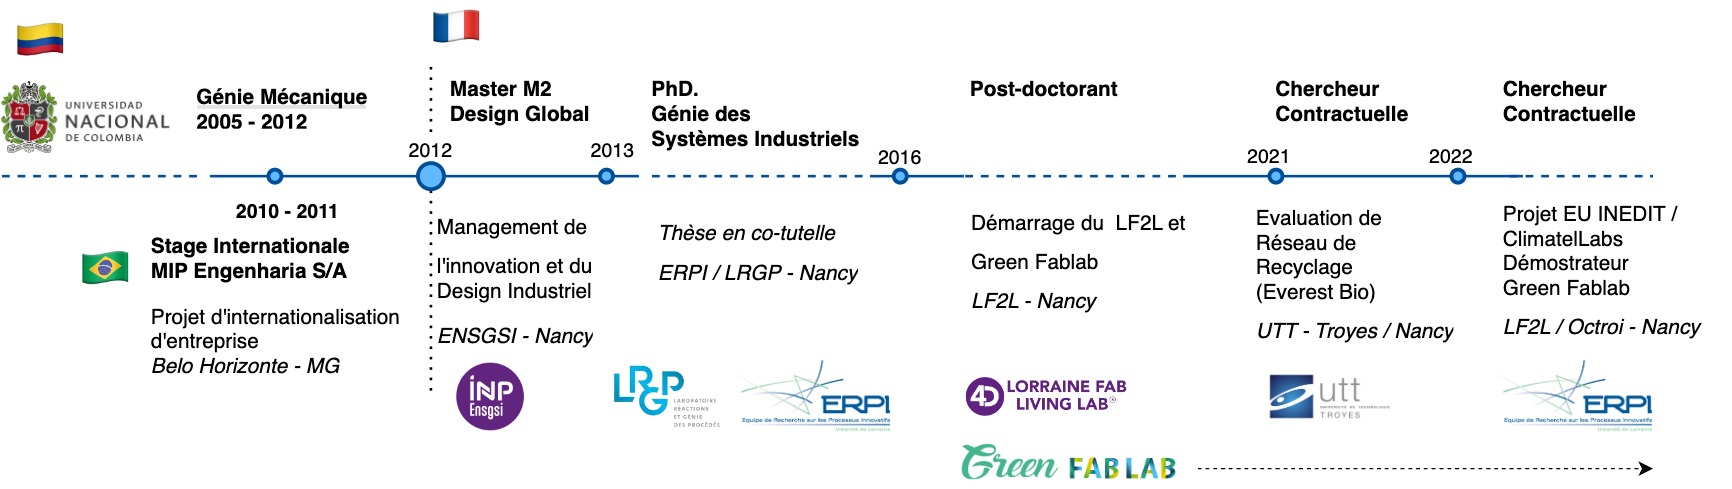
\includegraphics{Figures/slides/Fabio-timeline-Parcours.jpg}
\end{column}
\end{columns}

\note{}
\end{frame}

\hypertarget{activituxe9s-de-recherche}{%
\subsection{Activités de Recherche}\label{activituxe9s-de-recherche}}

\begin{frame}[t]{Domaine de recherche}
\protect\hypertarget{domaine-de-recherche}{}
\emph{Recyclage distribué} via open Source hardware: Validation
multi-echelle.

\begin{columns}[T]
\begin{column}[c]{0.6\textwidth}
\begin{enumerate}
\tightlist
\item
  Feasabilité technique
\item
  Filière en circuit court
\item
  (E)valuation sur le territoire
\end{enumerate}

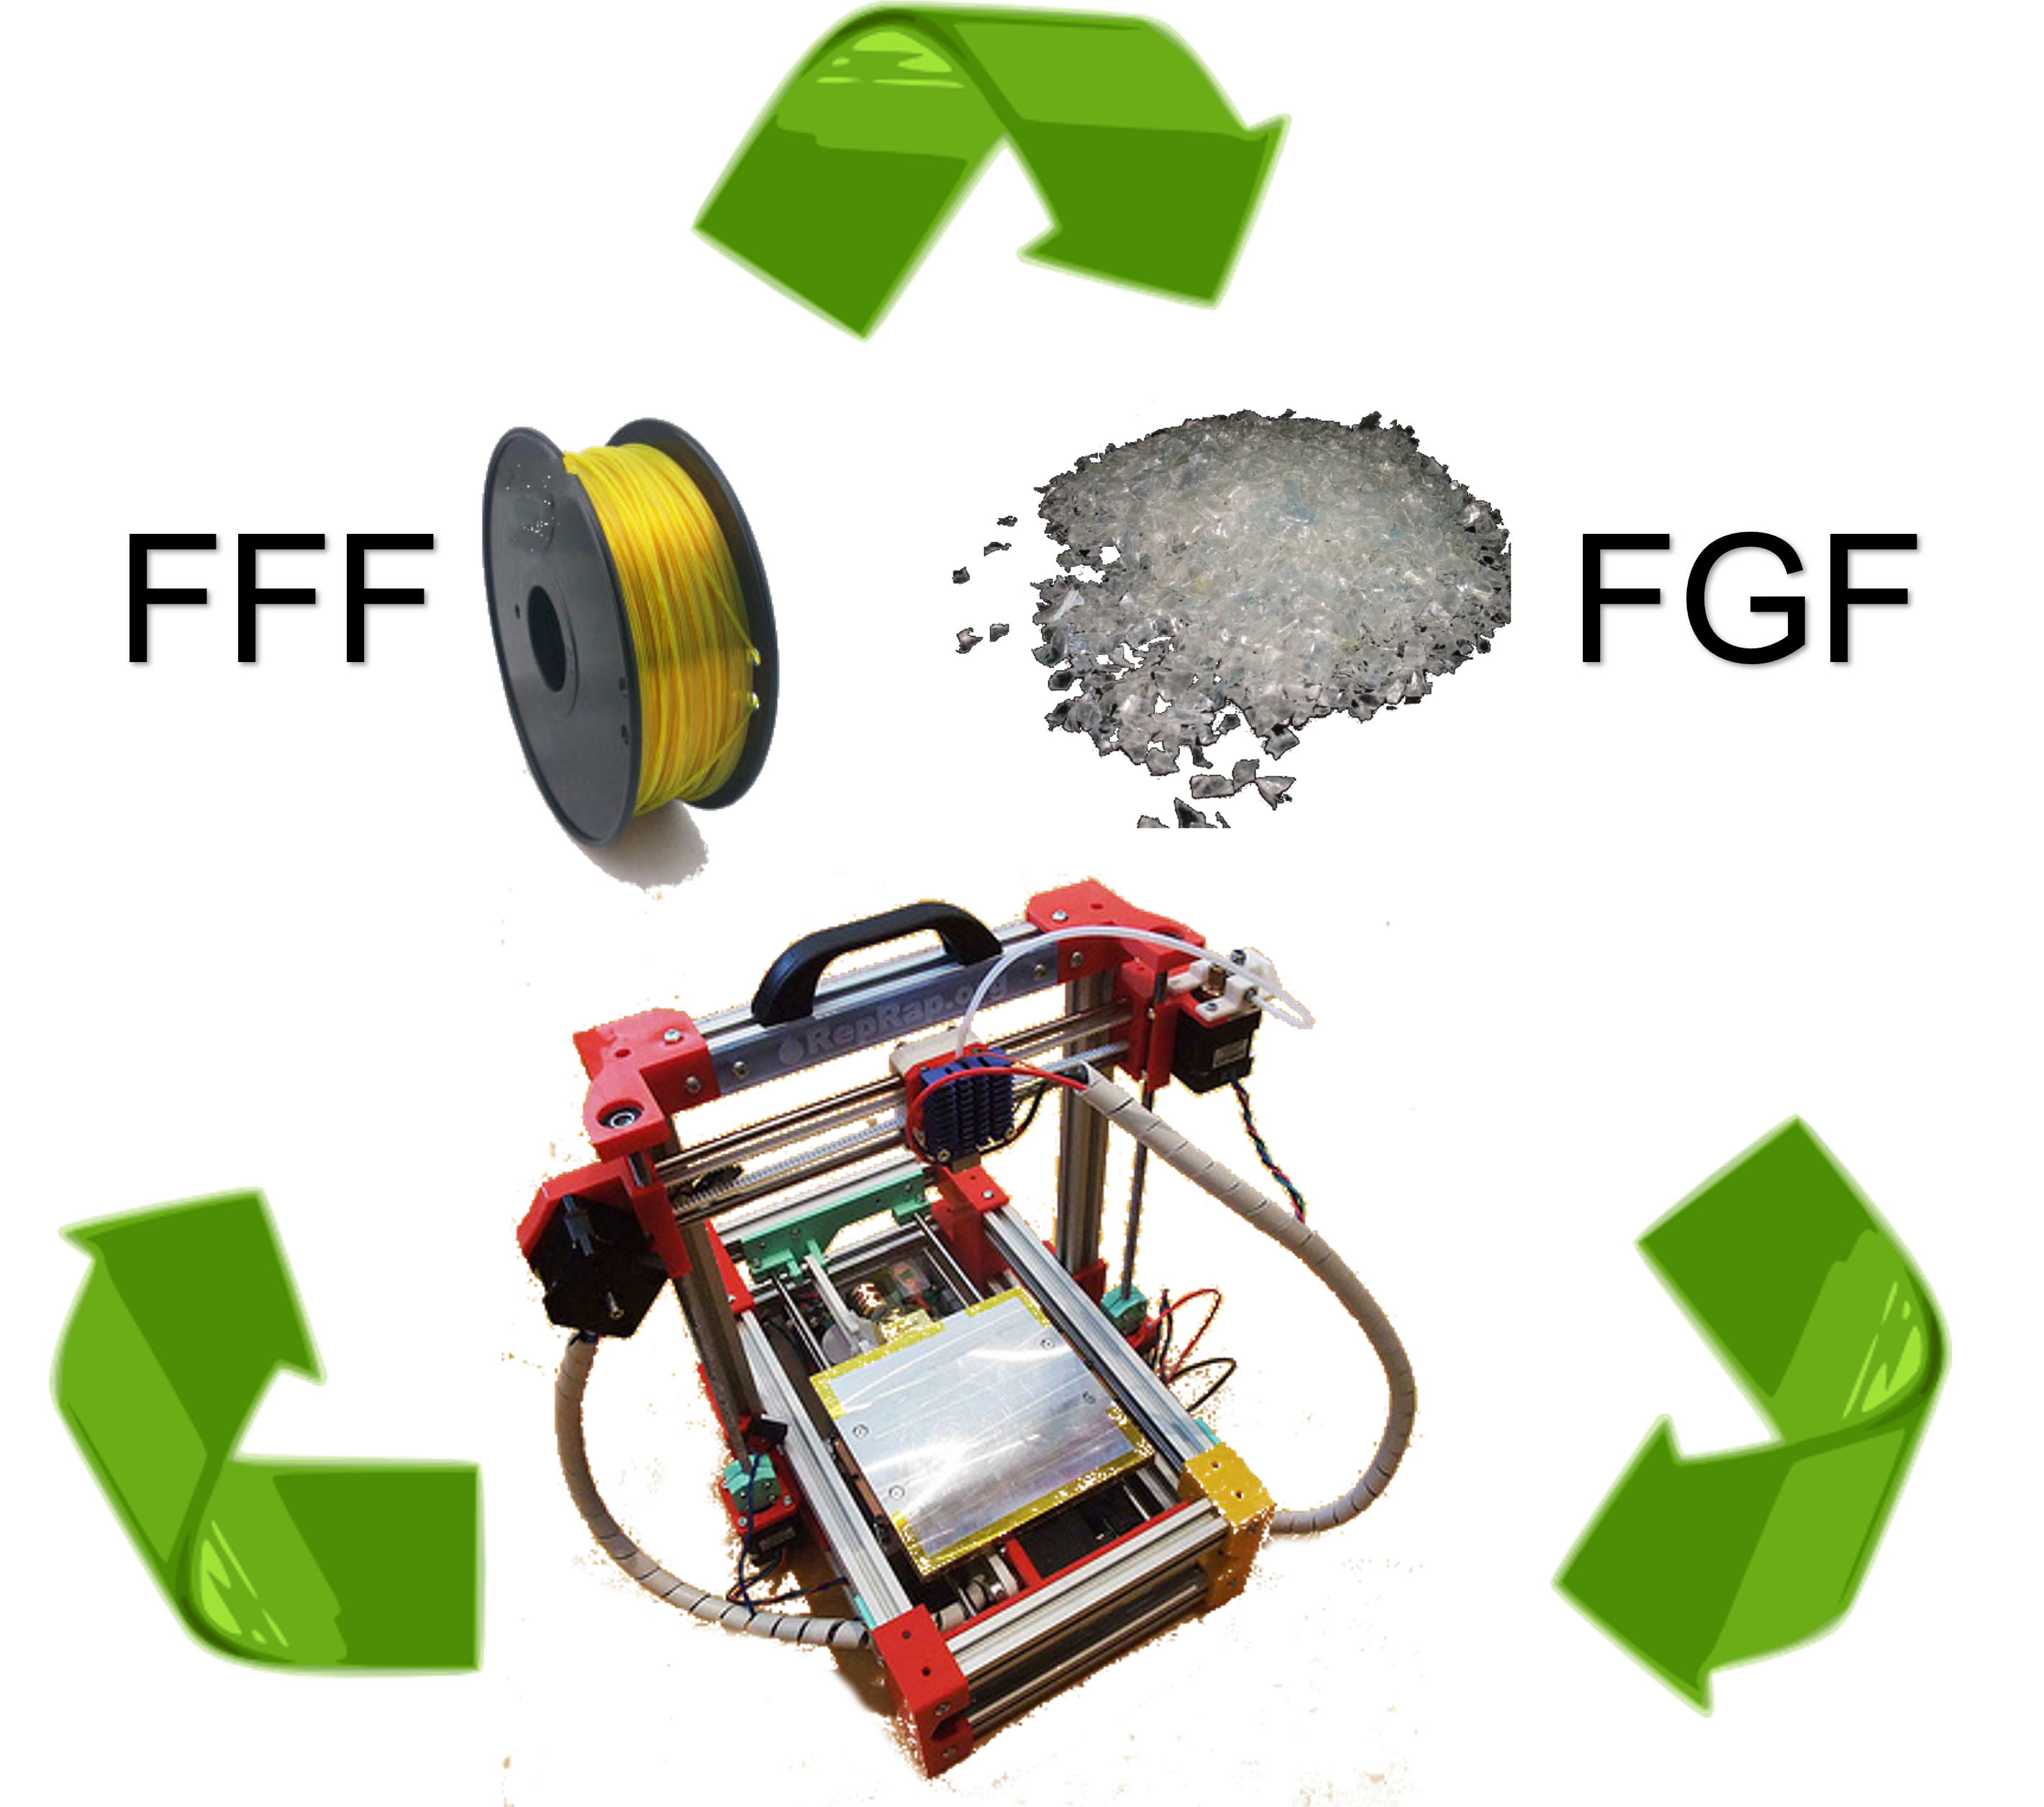
\includegraphics[width=1.04167in,height=\textheight]{Figures/slides/Recherche-Intro-01.png}
\end{column}

\begin{column}[c]{0.4\textwidth}
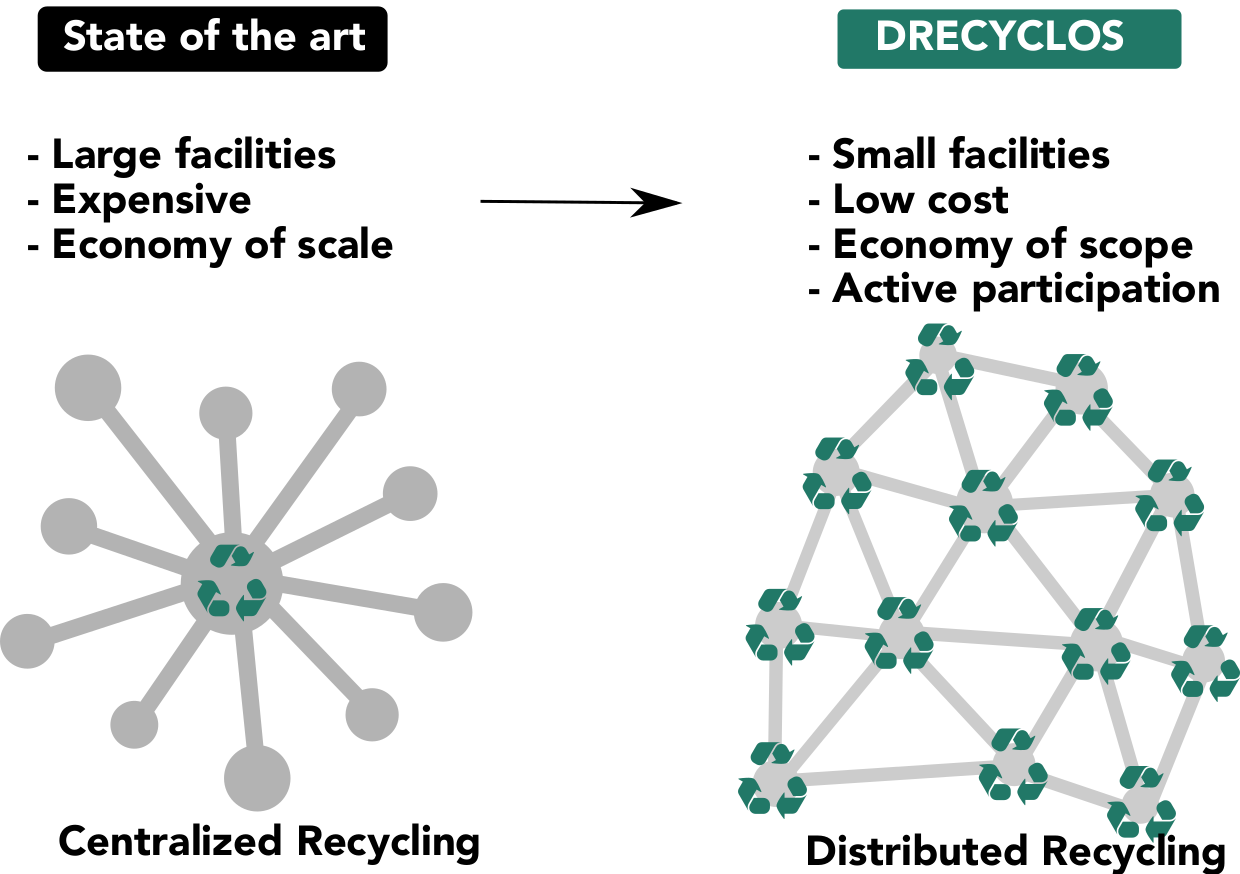
\includegraphics[width=2.60417in,height=\textheight]{Figures/slides/Abstract.png}
\end{column}
\end{columns}

\note{}
\end{frame}

\begin{frame}[t]{Axes de Recherche}
\protect\hypertarget{axes-de-recherche}{}
\emph{Recyclage distribué} via open Source hardware: \textbf{Validation
multi-echelle}

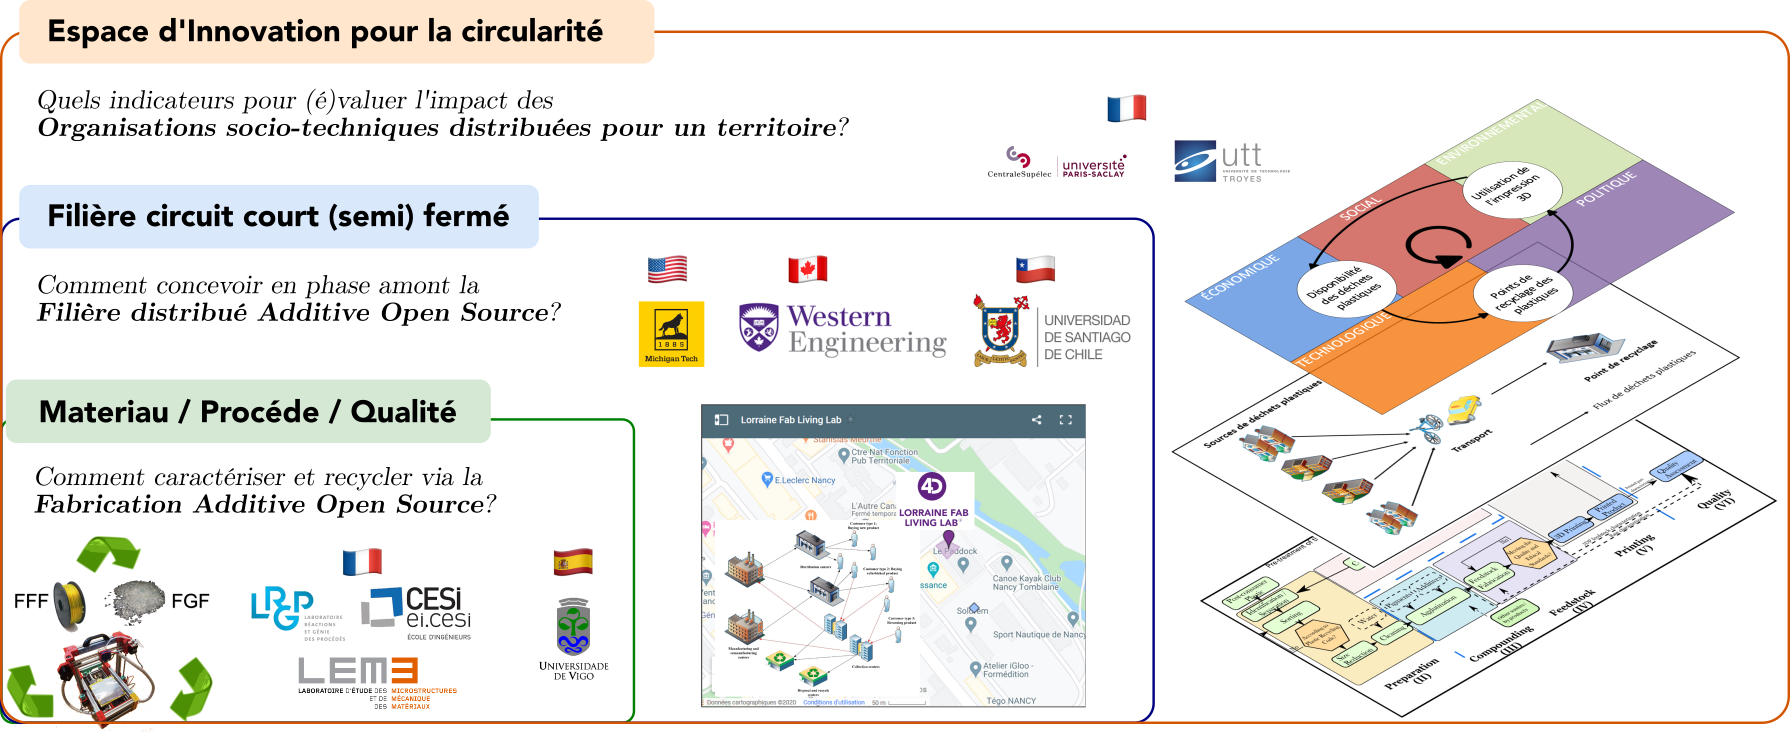
\includegraphics[width=0.9\textwidth,height=\textheight]{Figures/slides/recherche-fabio.png}

\note{Passon à mes activités de recherche.

Je m'interesse à la notion de Recyclage distribuée}
\end{frame}

\begin{frame}{Production Scientifique}
\protect\hypertarget{production-scientifique}{}
\begin{columns}[T]
\begin{column}[c]{0.3\textwidth}
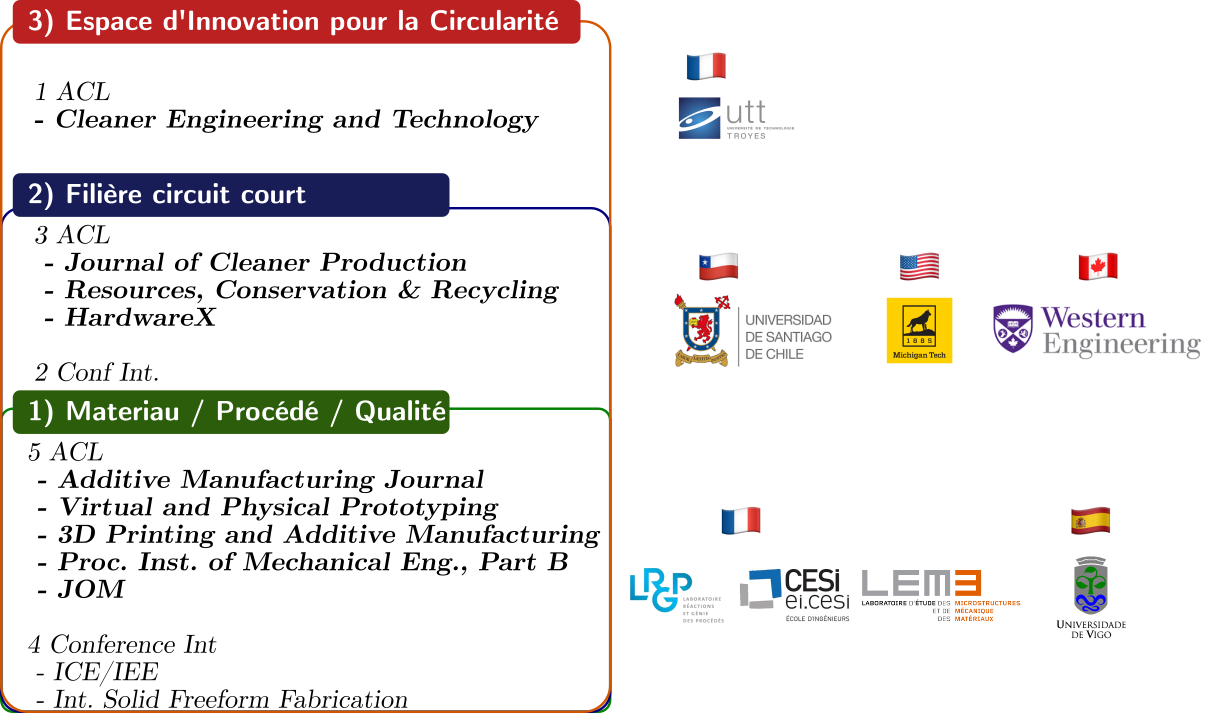
\includegraphics{Figures/slides/Journals/Journals.png}
\end{column}

\begin{column}[c]{0.58\textwidth}
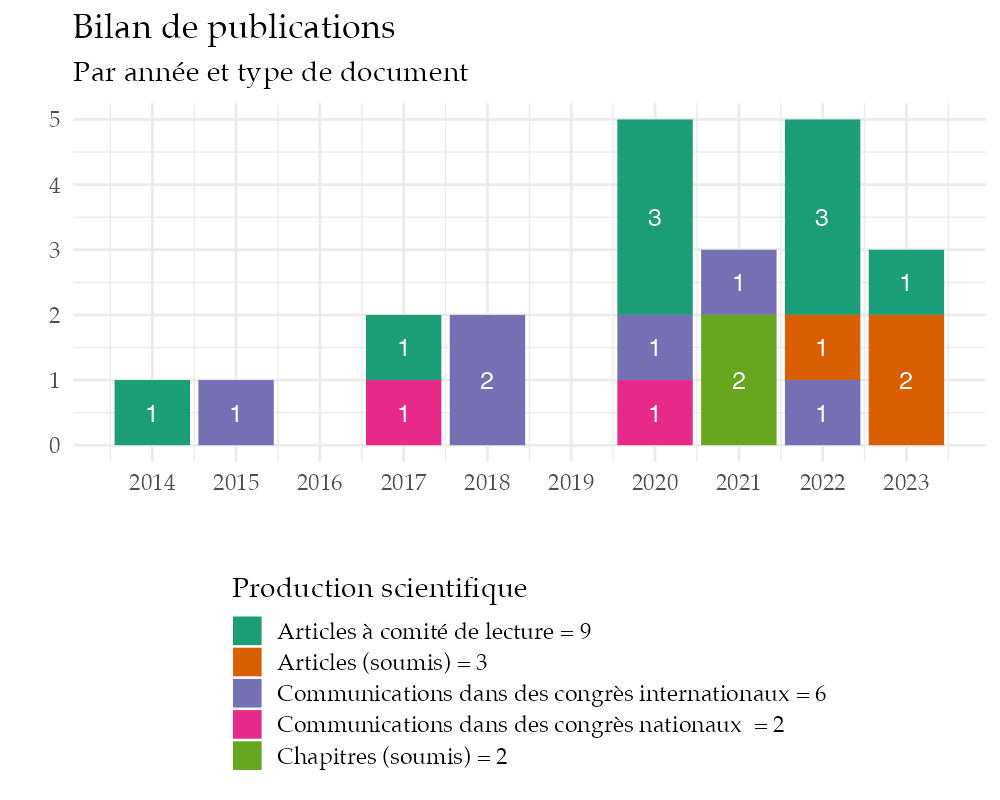
\includegraphics{Figures/slides/Fabio-Articles.jpg}
\end{column}
\end{columns}
\end{frame}

\begin{frame}{Participation DE Projets}
\protect\hypertarget{participation-de-projets}{}
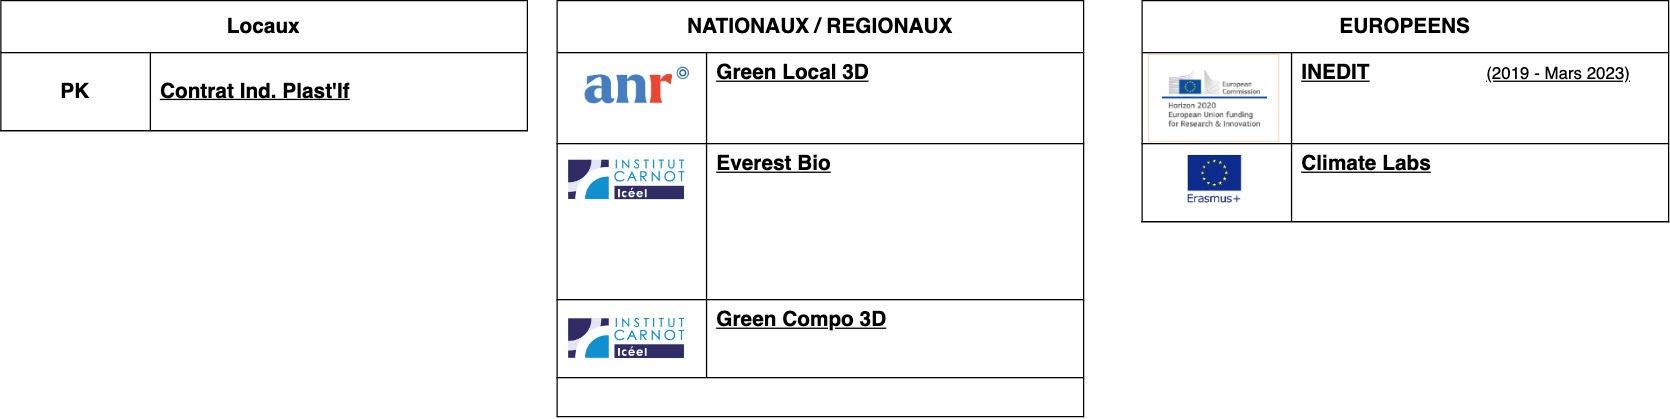
\includegraphics[width=0.8\textwidth,height=\textheight]{Figures/slides/Projects.jpg}
\end{frame}

\hypertarget{activituxe9s-denseignement}{%
\subsection{Activités d'Enseignement}\label{activituxe9s-denseignement}}

\begin{frame}{Synthèse quantitative des activités d'Enseignement}
\protect\hypertarget{synthuxe8se-quantitative-des-activituxe9s-denseignement}{}
\begin{columns}[T]
\begin{column}[c]{0.6\textwidth}
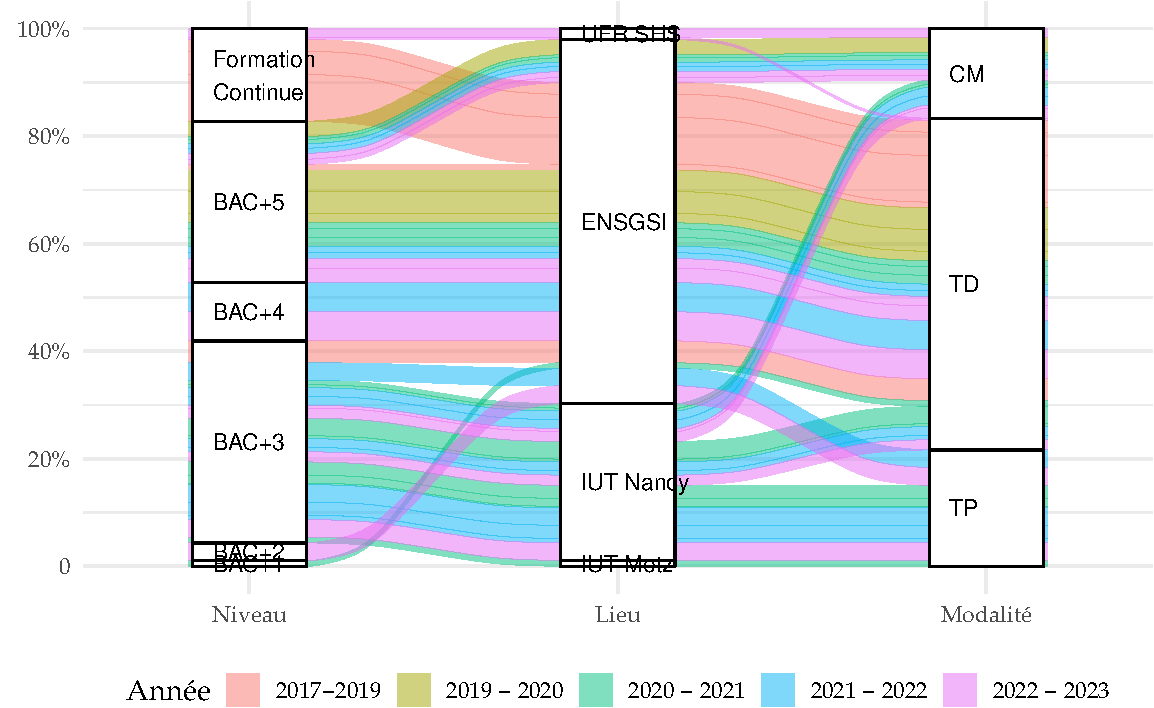
\includegraphics{figures/fig-sankey-1.pdf}
\end{column}

\begin{column}[c]{0.4\textwidth}
\begin{itemize}
\item
  Enseignements depuis 2017 : \textbf{386.92 h}
\item
  Pole Conception et Innovation
\end{itemize}
\end{column}
\end{columns}
\end{frame}

\begin{frame}[t]{Module CI15 - Recherche, Developpement et Innovation}
\protect\hypertarget{module-ci15---recherche-developpement-et-innovation}{}
\begin{columns}[T]
\begin{column}[c]{0.5\textwidth}
\scriptsize

\textbf{Objectif:}

\begin{itemize}
\tightlist
\item
  Recherche an tant que compétence transversal.
\item
  Lien entre la \textbf{recherche et leur sujet de stage!}.
\item
  Devenir un interlocuteur valable via la recherche.
\end{itemize}
\end{column}

\begin{column}[c]{0.5\textwidth}
\scriptsize

\begin{itemize}
\tightlist
\item
  Niveau BAC+5: ENSGSI 3AI, Master M2 IDEAS \& IUVTT
\end{itemize}
\end{column}
\end{columns}

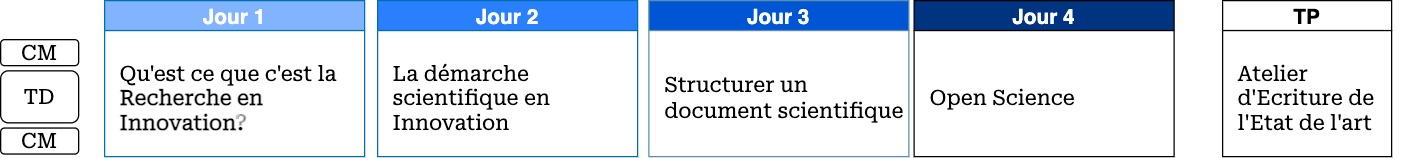
\includegraphics{figures/slides/Ensegnement-CI15.jpg}
\end{frame}

\begin{frame}{Licence After}
\protect\hypertarget{licence-after}{}
\begin{columns}[T]
\begin{column}[c]{0.6\textwidth}
\scriptsize

\textbf{Objectif:}

\begin{itemize}
\tightlist
\item
  Maîtriser et s'approprier les notions clés du recyclage
\item
  Prendre en main les outils de Green Fablab.
\item
  Impliquer les étudiants dans une démarche de construction pédagogique
\end{itemize}
\end{column}

\begin{column}[c]{0.4\textwidth}
\scriptsize

\begin{itemize}
\tightlist
\item
  Niveau BAC+2: Licence
\end{itemize}
\end{column}
\end{columns}

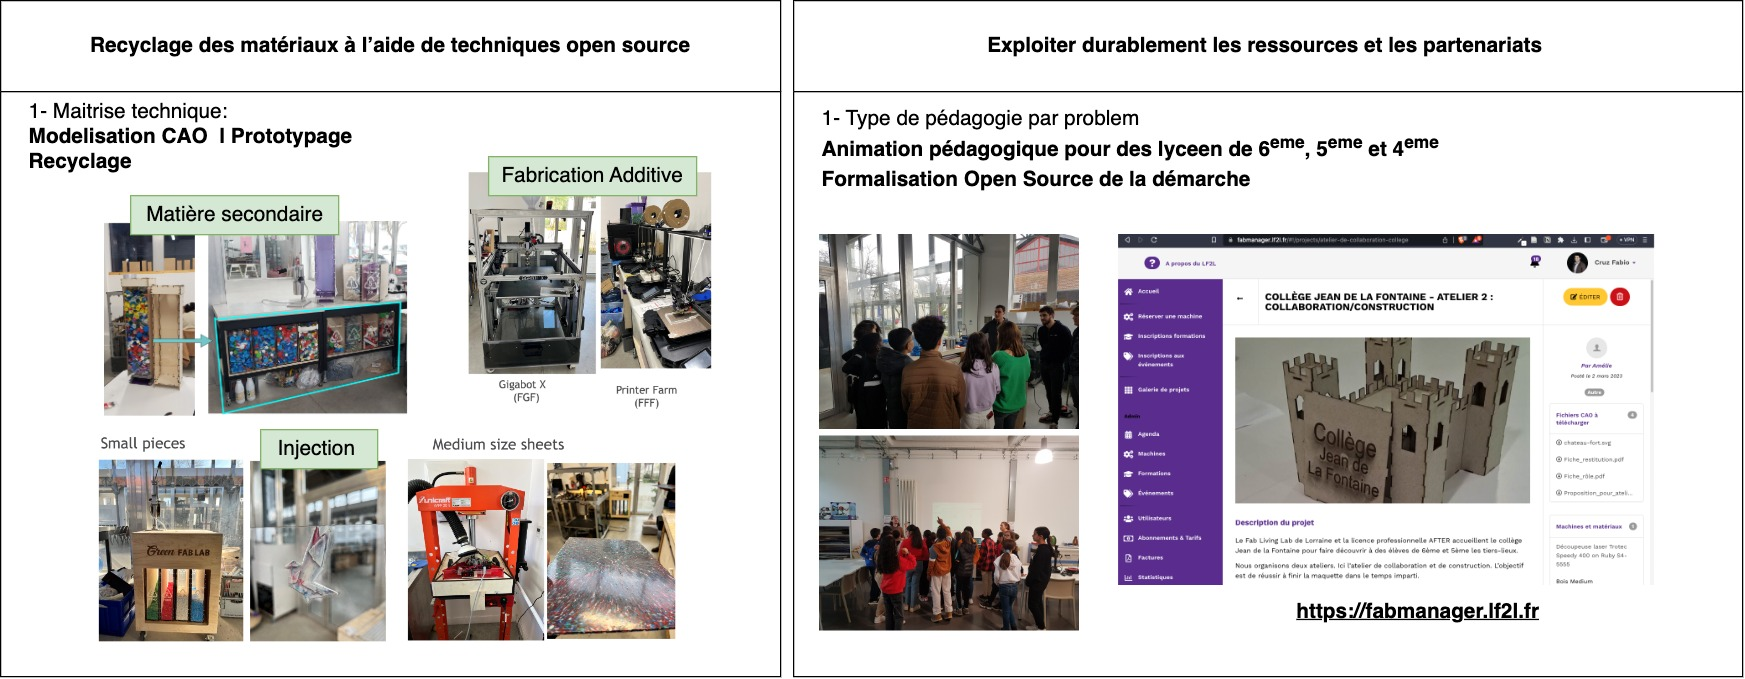
\includegraphics[width=0.9\textwidth,height=\textheight]{figures/slides/Ensegnement-AFTER.jpg}
\end{frame}

\hypertarget{proposition-dintuxe9gration-uxe0-lensgsi-et-uxe0-lerpi}{%
\section{Proposition d'intégration à l'ENSGSI et à
l'ERPI}\label{proposition-dintuxe9gration-uxe0-lensgsi-et-uxe0-lerpi}}

\hypertarget{ma-comprehension-de-lerpi-et-de-lensgsi}{%
\subsection{Ma comprehension de l'ERPI et de
l'ENSGSI}\label{ma-comprehension-de-lerpi-et-de-lensgsi}}

\begin{frame}{Ma comprehension de l'ERPI et de l'ENSGSI}
\footnotesize

\begin{columns}[T]
\begin{column}[T]{0.5\textwidth}
ENSGSI

\begin{itemize}
\item
  Ingénieurs généralistes d'envergure internationale.
\item
  Génie industriel -\textgreater{} Ingénierie de l'Innovation.
\item
  Secteurs d'activités : énergie, environnement, développement durable,
  cosmétique, design de produits et services.
\end{itemize}
\end{column}

\begin{column}[T]{0.5\textwidth}
ERPI

\begin{itemize}
\item
  Nouvelles méthodologies pour soutenir et fiabiliser les processus
  d'innovation (technologiques, organisationnelles, ou sociales).
\item
  Faciliter la prise de décision des parties prenantes.
\item
  Thèmes de recherche:

  \begin{itemize}
  \tightlist
  \item
    Aide à la conception en amont
  \item
    Acceptabilité du produit, du processus et de la filière
  \end{itemize}
\end{itemize}
\end{column}
\end{columns}

\large

Develpper une *Génie de l'Innovation Eco-Responsable**

\normalsize
\end{frame}

\hypertarget{projet-de-recherche}{%
\subsection{Projet de Recherche}\label{projet-de-recherche}}

\begin{frame}{Projet de Recherche}
Green Fablab comme projet federateur et transversal pour ERPI:

\begin{columns}[T]
\begin{column}[T]{0.3\textwidth}
\footnotesize

\begin{itemize}
\item
  Nouveaux démonstrateurs et protocoles expérimentaux Open Source
\item
  Recherche fondamental vers Recherche-action
\item
  (E)valuation Multi-acteurs et Multi-echelle
\end{itemize}
\end{column}

\begin{column}[T]{0.7\textwidth}
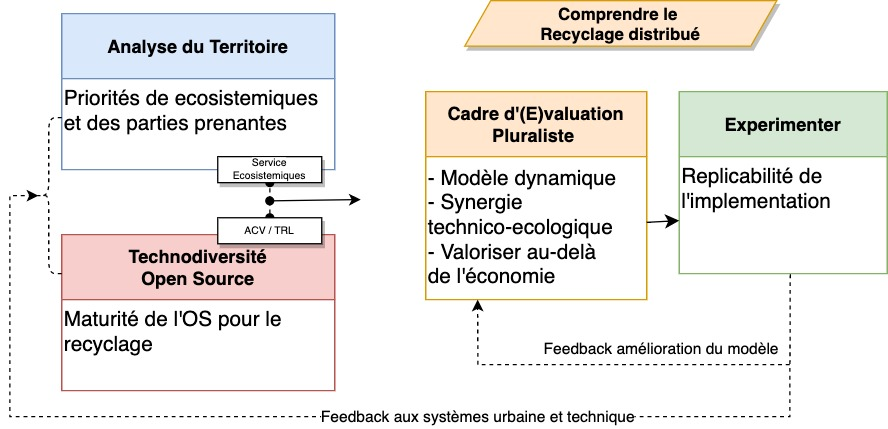
\includegraphics{Figures/slides/Projet-Recherche.jpg}
\end{column}
\end{columns}
\end{frame}

\hypertarget{projet-pedagogique}{%
\subsection{Projet Pedagogique}\label{projet-pedagogique}}

\begin{frame}{Ma vision de la pédagogique}
\protect\hypertarget{ma-vision-de-la-puxe9dagogique}{}
L'ambition que je porte avec l'enseignement:

\begin{itemize}
\item
  Developper des contenus pédagogiques favorisant l'expérimentation DIY
\item
  Faciliter la manipulation des concepts
\item
  Faire le lien avec les enjeux societaux et leur parcours Ingénieur
\end{itemize}
\end{frame}

\begin{frame}{Les axes pedagogiques que je peux apporter}
\protect\hypertarget{les-axes-pedagogiques-que-je-peux-apporter}{}
\begin{enumerate}
\item
  La compréhension de la caractérisation des matériaux en utilisant
  l'approche open hardware comme support pédagogique
\item
  La conception de produit en utilisant des critères de soutenabilité
  tels que la réparabilité, le recon- ditionnement et le recyclage.
\item
  L'open source comme une pratique disruptive dans la conception
  mécanique et dans l'innovation produit.
\end{enumerate}
\end{frame}

\begin{frame}{Integration dans la maquette actuel}
\protect\hypertarget{integration-dans-la-maquette-actuel}{}
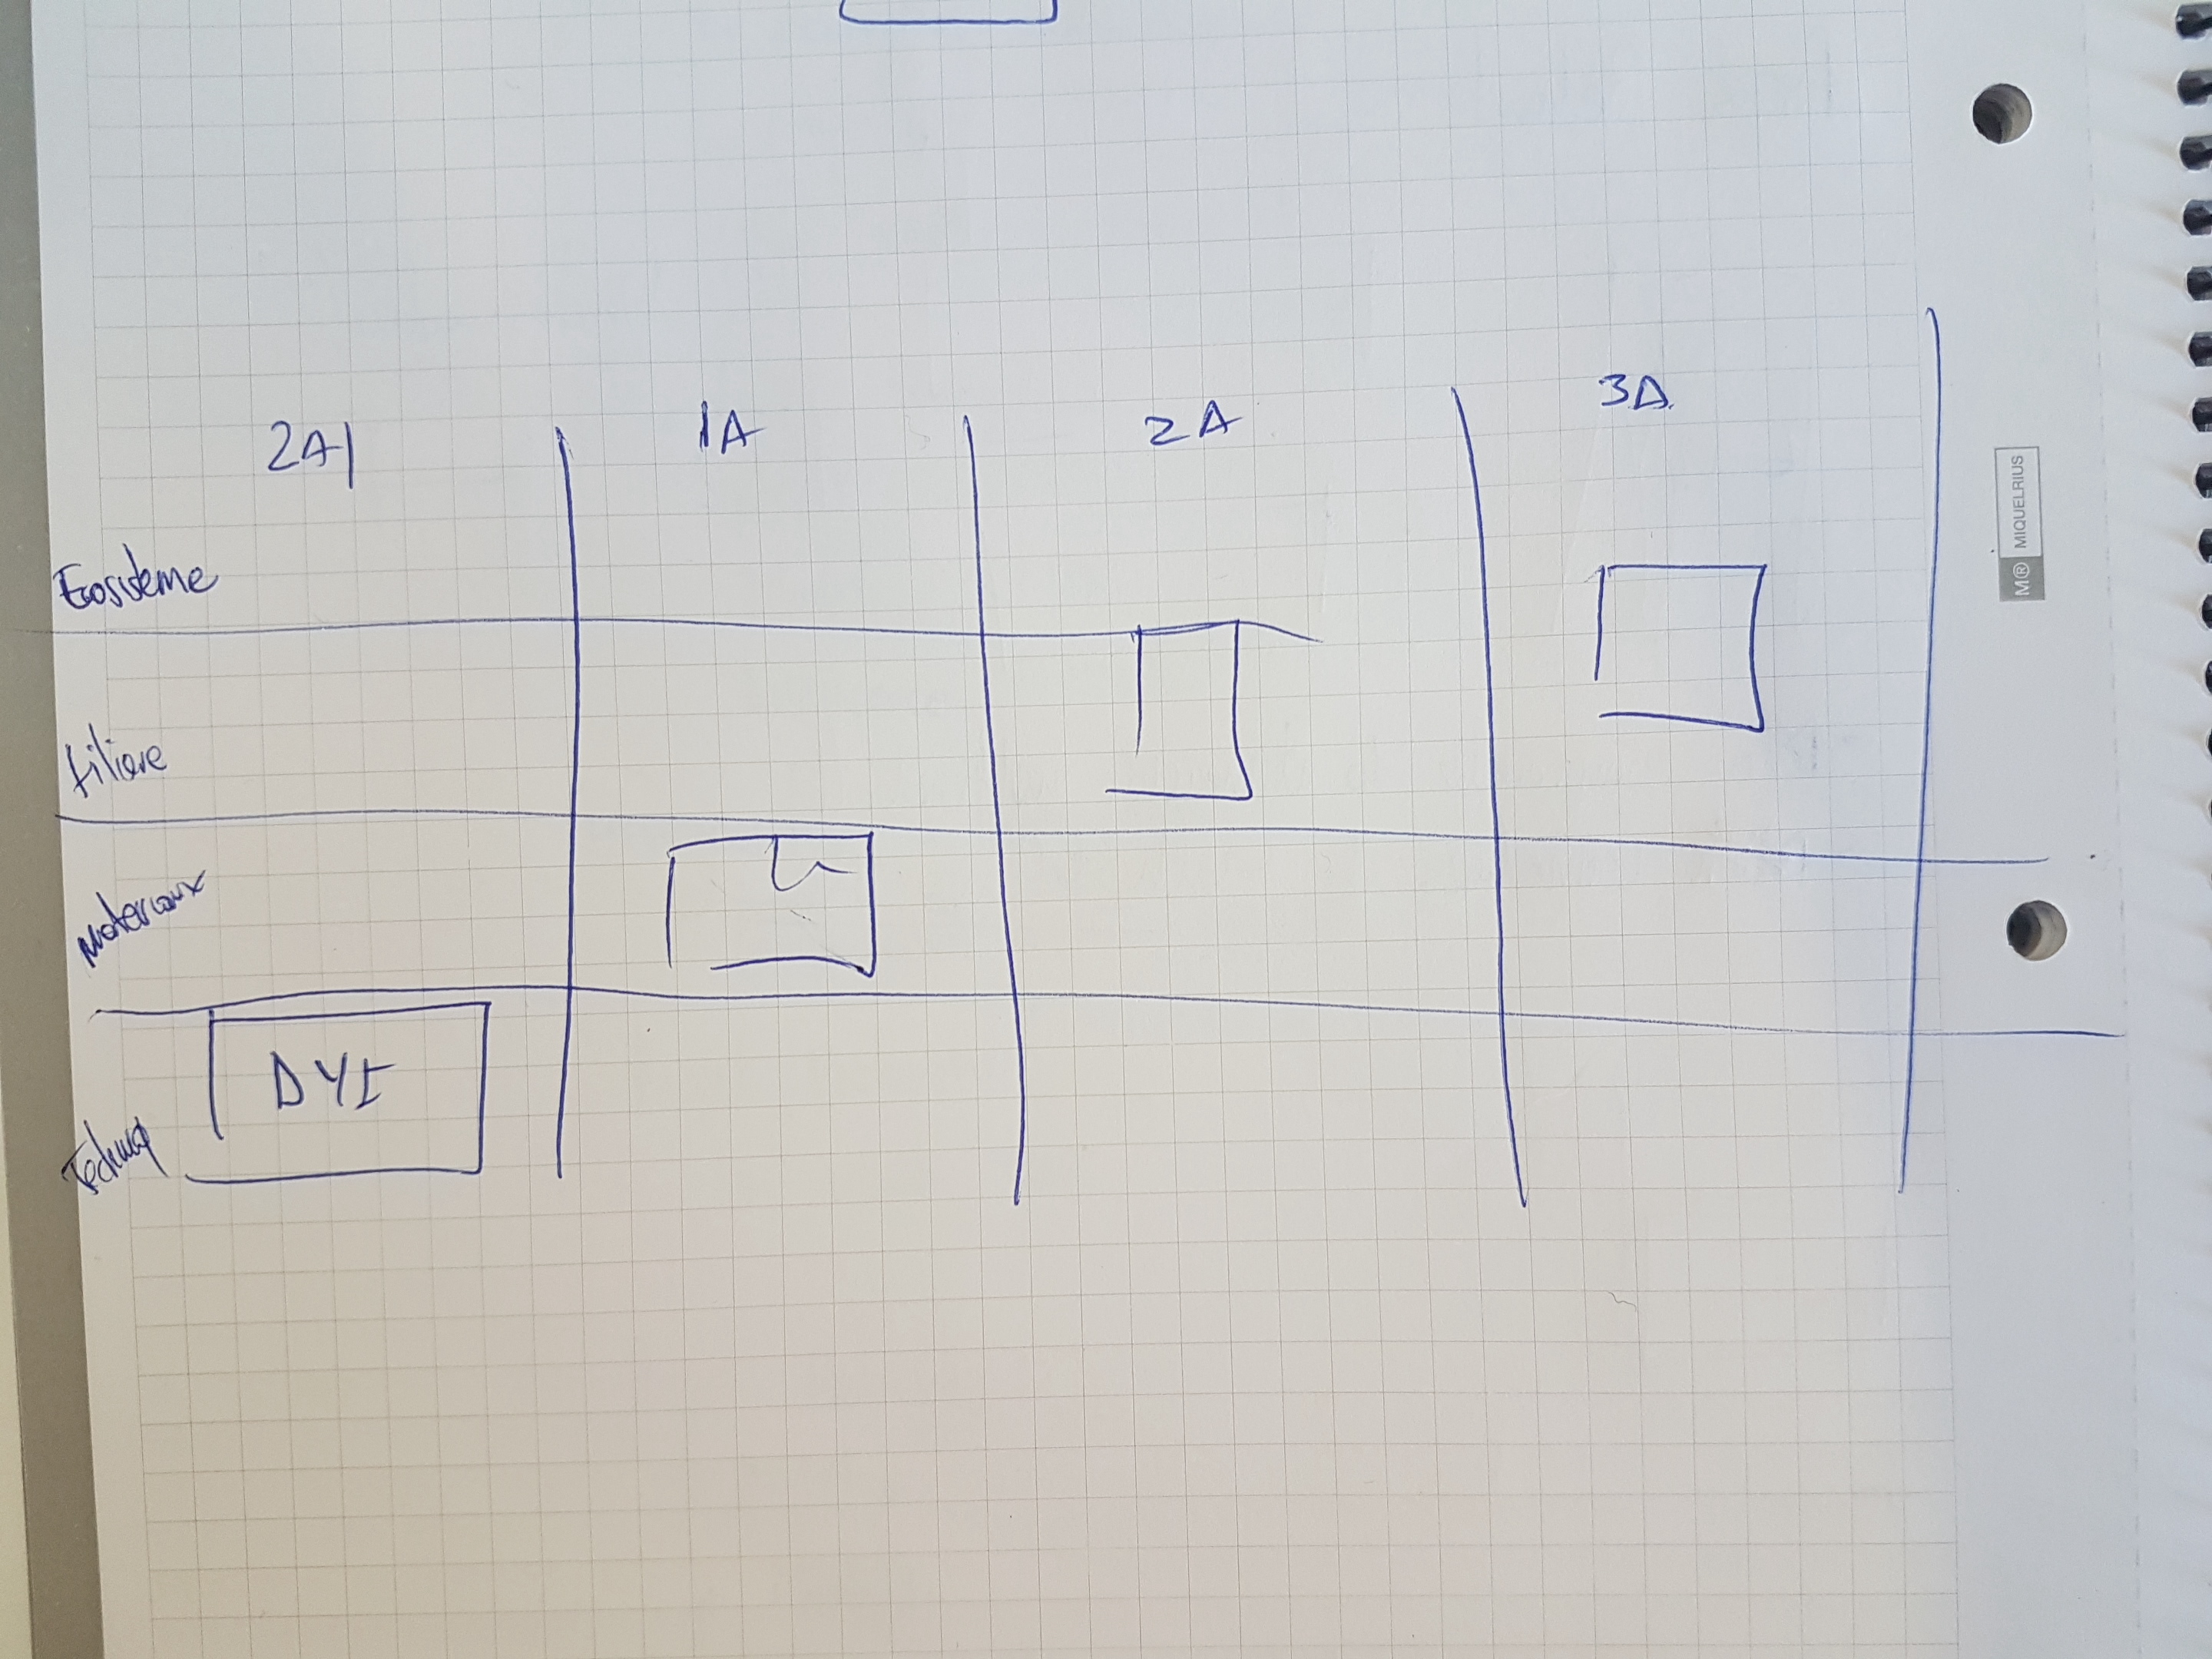
\includegraphics{figures/slides/Projet-pedagogique.jpg}
\end{frame}

\begin{frame}{Example en cours: TP Age du Faire et du DIY \hfill 2AP
ENSGSI}
\protect\hypertarget{example-en-cours-tp-age-du-faire-et-du-diy-2ap-ensgsi}{}
\begin{itemize}
\tightlist
\item
  Proposition de TP de 6h pour faire le lien entre recherche et
  pédagogique
\item
  Valorisation pédagogique du projet recherche INEDIT
\end{itemize}

{[}Photo TP?{]}
\end{frame}

\hypertarget{responsabilituxe9s-collectifs-actuel-et-futur}{%
\subsection{Responsabilités Collectifs (Actuel et
futur)}\label{responsabilituxe9s-collectifs-actuel-et-futur}}

\begin{frame}{Responsabilités Collectifs (Actuel et futur)}
\begin{block}{Vie du Laboratoire}
\protect\hypertarget{vie-du-laboratoire}{}
\scriptsize

\begin{itemize}
\tightlist
\item
  Pilote des projets en lien avec le Green Fablab.
\item
  Support au LF2L et ERPI dans site web / numerique.
\item
  Travail collaboratif avec les chercheurs du laboratoire et d'autres
  laboratoires dans des projets interdisciplinaires
\item
  Montage de projets de recherche (EU, Nationaux)
\end{itemize}
\end{block}

\begin{block}{Vie de l'Ecole}
\protect\hypertarget{vie-de-lecole}{}
\scriptsize

\begin{itemize}
\tightlist
\item
  Animation de séances de prototypage dans le cadre d'évènements
  organisés par l'école
\item
  Implication dans les journées Portes Ouvertes
\item
  Lien avec Green Fablab et le territoire via l'Octroi.
\item
  Prix de `Coup de Coeur' de \textbf{Campus Responsable}
\end{itemize}
\end{block}

\begin{block}{Animation scientifique, vulgarisation}
\protect\hypertarget{animation-scientifique-vulgarisation}{}
\scriptsize

\begin{itemize}
\tightlist
\item
  Participation à la finale régionale de «\emph{Ma thèse en 180
  secondes}»
\item
  Participation à la foire internationale de Nancy
\item
  Conferences grand public au LF2L
\end{itemize}
\end{block}
\end{frame}

\hypertarget{conclusion}{%
\section{Conclusion}\label{conclusion}}

\hypertarget{mon-approt-pour-la-recher}{%
\subsection{Mon approt pour la Recher}\label{mon-approt-pour-la-recher}}

\begin{frame}{Mon approt pour la Recher}
\begin{enumerate}
\tightlist
\item
  Apporter mes compétences pour un plus grande compréhension des
  \textbf{leviers socio-techniques}. C'est-à-dire l'étude simultanée des
  facteurs technico-économiques, et sociales qui sont nécessaires pour
  l'accélération vers transitions soutenabilité de l'industrie (economie
  circulaire, )
\end{enumerate}

\begin{itemize}
\tightlist
\item
  Contribuer aux projets du laboratoire, principalement sur la notion de
  filière à travers la conception, l'évaluation, l'optimisation, la
  démonstration et la gestion
\end{itemize}

Mettre en place des collaborations avec différents laboratoires, des
collectivités et des entreprises

\appendix
\end{frame}

\hypertarget{appendix}{%
\section{appendix}\label{appendix}}

\begin{frame}[t]{Domaine de recherche}
\protect\hypertarget{domaine-de-recherche-1}{}
\emph{Recyclage distribué} via open source hardware: Validation
multi-echelle.

\begin{enumerate}
\tightlist
\item
  Feasabilité technique
\item
  Filière en circuit court
\item
  (E)valuation sur le territoire
\end{enumerate}

\begin{tikzpicture}[remember picture,overlay]
    \node[xshift=1.5cm,yshift=-1.3cm] at (current page.center) {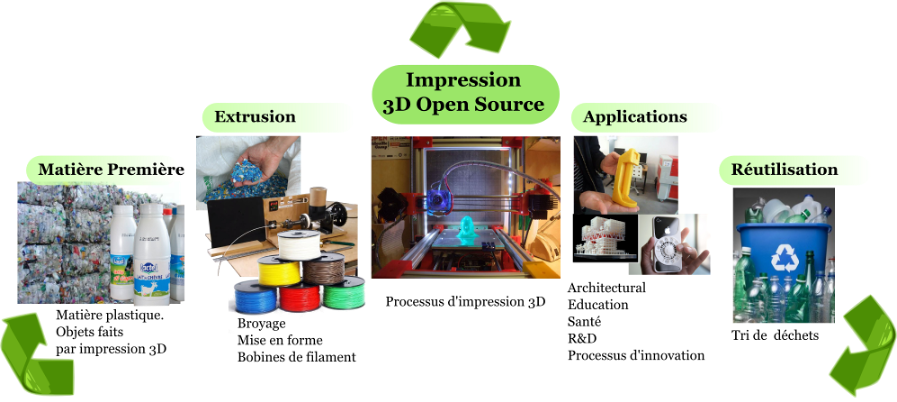
\includegraphics[width=12cm]{Figures/slides/DRAM-00.png}};
\end{tikzpicture}

\note{}
\end{frame}



\end{document}
